\documentclass[UTF8]{ctexart}

\ctexset{
	section = {
		format+ = \zihao{4} \heiti \centering
	},
	subsection ={
		format+ = \zihao{-4} \heiti \raggedright
	},
	subsubsection = {
		format+ = \zihao{-4} \heiti \raggedright
	}
}
\pagestyle{plain}
\usepackage{float}
\usepackage{graphicx}
\usepackage{amsmath}
\usepackage{amsthm}
\newtheorem{pro}{定理}
\graphicspath{{figures/}}
\usepackage{subfigure}
\usepackage{appendix}
\usepackage{amssymb}
\usepackage{setspace}
\usepackage{url}
\usepackage{booktabs}
\usepackage{geometry}
\geometry{left=3cm,right=3cm,top=2.54cm,bottom=2.54cm}

\linespread{1.3}

\begin{document}
	
	%	\setlength{\baselineskip}{20pt}
	\zihao{-4} \songti
	
	\tableofcontents
	\newpage
	
	\section{问题重述}
	各国为控制疫情研发新冠疫苗。若干种疫苗需要顺序经过若干个工位生产。考虑到疫苗在不同工位生产的时间和顺序,我们需要根据疫苗生产的条件和要求,对不同环境的疫苗生产进行建模,以保证疫苗生产的高效性和有序性。
	
	首先疫苗生产有严格的限制条件:同一类型100剂疫苗为一箱进行处理;每种疫苗按照CJ1-CJ2-CJ3-CJ4的顺序在4个工位进行了加工;每个工位不能同时生产不同类型的疫苗,疫苗生产不允许插队,即进入第一个工位安排的每类疫苗的生产顺序决定整体生产顺序。其次有YM1-YM10等10种不同类型的疫苗需要生产。
	
	考虑以上影响因素,我们需要解决以下问题。
	
	\textbf{问题一:}
	对每箱疫苗在所有工位上的生产时间进行均值、方差、最值、概率分布等统计分析,掌握每个工位生产疫苗的能力水平。
	
	\textbf{问题二:}
	在最短时间内,生产YM1-YM10各100剂疫苗,建立数学模型,求出疫苗生产的顺序和生产总时间,并将结果填入表1。
	
	\textbf{问题三:}
	考虑疫苗实际生产时间的随机性。要求总时间比问题2给定的最短时间缩短5\%,建立数学模型,以最大的概率完成这个任务为目标,确定生产顺序,并给出缩短的时间比例与最大概率之间的关系。
	
	\textbf{问题四:}
	附件2中规定了不同规模的10种类型的生产任务。在每个每个工位每天生产的时间不能超过16小时和每种类型疫苗的生产任务不可以拆分的情况下,建立数学模型,使得可靠性为90\%,求出完成任务的最少天数。
	
	\textbf{问题五:}
	对于附件2中的疫苗生产任务,在生产时间限制在100天内、每个工位每天生产的时间不能超过16小时和每种类型疫苗的生产任务可以适当拆分的情况下,建立数学模型,安排生产计划,使得销售额达到最大值。
	
	\section{问题分析}
	\textbf{对问题一的分析:}问题一要对多组数据进行多种统计分析,考虑数据处理的方便性,我们先对数据进行预处理,采取部分数据确定其概率分布方式,再定义一个求取一组数据均值、方差、最值和确定分布方式的函数,最后使用函数对每组数据进行统计分析。
	
	\textbf{对问题二的分析:}问题二要制定疫苗的生产顺序和计算生产总时间。考虑到题目中的加工工位顺序和生产不允许排队的限制条件是非线性的,因此可以先用程序搜索出满足要求的可行的生产方案,从而解除非线性约束。根据可行的生产方案,我们采用启发式算法搜索最优解,即最短生产时间,并不断检查是否满足剩余的两项的限制条件,注意记录最优解的疫苗生产顺序。
	
	\textbf{对问题三的分析:}问题三要制定缩短时间下最大概率疫苗的生产顺序,以及给出缩短的时间比例与最大概率之间的关系。在问题二的基础上,将约束条件改成生产时间缩短5\%,用程序搜索满足对应的条件的可行方案,再采用启发式算法求最优解,但与问题二不同,最优解改成求最大概率,并注意记录最优解的疫苗产生顺序。启发式算法求最优解的过程,同样也是求最大概率与缩短时间的关系。
	
	\textbf{对问题四的分析:}问题四要求出完成任务可靠性为90\%的最少天数。仍是涉及流水线的非线性优化问题,约束条件增加为每种类型疫苗的生产任务不可拆分和在可靠性为90\%的前提下。所以为了简便求解,我们这一题的重点不在细节地通过生产顺序来计算流水线平衡目标。目标函数不采用多个独立事件的概率乘法公式作为,即不以每天每工位生产的可靠性作为独立事件,而是根据正态分布特性使用概率和微分方程进行整体求解得到可靠性90\%的最大总时间。
	
	
	\textbf{对问题五的分析:}问题五求在若干非线性约束条件下使得最大销售和疫苗生产顺序和产量。约束条件修改为生产时间限制在100天内、每个工位每天生产的时间不能超过16小时和每种类型疫苗的生产任务可以适当拆分。我们选择对多个约束条件进行拆分简化,先固定其中一个参数产量,使问题变为线性优化。根据求解线性组合得到的结果进行不同疫苗产量的百分比和优先级。百分比和优先级作为求另一个参数销售值的约束条件,采用与问题二和三相同的模拟退火算法求解,最优解改为最大销量,并不断检查是否满足剩余的两项的限制条件,注意记录最优解的疫苗生产顺序。
	
	
	\section{模型假设}
	为了简化问题,便于分析和求解,对模型进行以下合理的假设:
	\begin{enumerate}
		\item
	\end{enumerate}
	
	\section{定义和符号说明}
	%	\begin{table}[!ht]
	%		\caption{定义和符号说明表}\label{}
	%		\begin{tabular*}{\hsize}{@{}@{\extracolsep{\fill}} c c}
	%			\toprule[2pt]
	%			符号 & 说明   \\
	%			\hline
	%			&    \\
	%			&    \\
	%			&    \\
	%			\bottomrule[2pt]			
	%		\end{tabular*}		
	%	\end{table}
	\begin{table}[H]
	\centering
	\begin{tabular}{ c c c}
		\toprule[2pt]
		符号 & 说明  & 单位 \\
		\hline
		YM1$\sim$YM10 & 疫苗 & \\
		CJ1$\sim$CJ4 &  工位 &\\
		$T(i,j)$&  疫苗YM$i$在工位CJ$j$上生产耗时的随机变量&\\
		$\mu(i,j)$& $T(i,j)$的均值 &\\
		$\sigma(i,j)$ & 方差 &\\
		$T_{\Sigma}$ & 总用时 &\\
		$\alpha(i,j)$ & 加权系数 &\\
		$T_{W}$ & 等待时间 & b\\
		$M$ & 销售额 & \\
		$m_{i}$ & 疫苗$i$的单价 & \\
		$n_{i}$ & 疫苗$i$的产量 & \\
		$x_{k}$& 按顺序第$k$个被生产的疫苗& \\
		$\Omega_{in}(k,j)$& 第$k$个疫苗进入CJ$j$的时刻 & \\
		$\Omega_{out}(k,j)$& 第$k$个疫苗离开CJ$j$的时刻 & \\
		
		\bottomrule[2pt]
	\end{tabular}\caption{定义和符号说明}
\end{table}
	
	\section{数学基础}
	\subsection{正态分布}
	若连续型随机变量$X$的概率密度为
	\begin{equation}
	f(x)=\frac{1}{\sqrt{2\pi}\sigma}e^{-\frac{(x-\mu)^2}{2\sigma^2}}
	\end{equation}
	则称$X$服从参数为$\mu$,$\sigma$的正态分布,记为$X\sim\mathcal{N}(\mu,\sigma^2)$
	随机变量$X$的分布函数为
	\begin{equation}
	F(x)=\frac{1}{\sqrt{2\pi}\sigma}\int^{x}_{-\infty}e^{-\frac{(t-\mu)^2}{2\sigma^2}}dt
	\end{equation}
	\subsection{多元随机变量}
	多个相互独立的正态分布随机变量的线性组合也符合正态分布。
	
	为证明此结论,我们需要先证明两个相互独立的标准正态分布线性组合X+Y的服从正态分布,即:
	\begin{pro}
		设X,Y相互独立,$X\sim\mathcal{N}(\mu_{x},\sigma_{x}^2)$,$Y\sim\mathcal{N}(\mu_{y},\sigma_{y}^2)$,则X+Y服从正态分布,有$X+Y\sim\mathcal{N}(\mu_{x}+\mu_{y},\sigma_{x}^2+\sigma_{y}^2)$。
	\end{pro}

	\begin{proof}
		
	\end{proof}
	
	得到更一般的结论n个独立的正态分布的线性组合仍服从正态分布:
	
	\begin{pro}
		设$X_{1},X_{2},\cdots,X_n$相互独立,且$X_i\sim\mathcal{N}(\mu_{i},\sigma_{i}^2)$,$i=1,2,\cdots,n$,则有$X_{i}$的线性组合服从正态分布,即$C_1 X_1+C_2 X_2+\cdots +C_n X_n\sim\mathcal{N}(C_1\mu_1+C_2\mu_2+\cdots+C_n\mu_n,C_{1}^2\sigma_{1}^2+C_{2}^2\sigma_{2}^2+\cdots+C_{n}^2\sigma_{n}^2)$。
	\end{pro}
	
	
	\section{模型建立、求解和分析}
	\subsection{问题一}
	\subsubsection{数据的正态性检验}
	\begin{itemize}
		\item 偏度和峰度
		\begin{enumerate}
			\item 偏度:描述数据分布不对称的方向及其程度
			
			当偏度≈0时,可认为分布是对称的,服从正态分布;
			
			当偏度>0时,分布为右偏,即拖尾在右边,峰尖在左边,也称为正偏态;
			
			当偏度<0时,分布为左偏,即拖尾在左边,峰尖在右边,也称为负偏态;
			
			\item 峰度:描述数据分布形态的陡缓程度
			
			当峰度≈0时,可认为分布的峰态合适,服从正态分布(不胖不瘦);
			
			当峰度>0时,分布的峰态陡峭(高尖);
			
			当峰度<0时,分布的峰态平缓(矮胖);
			
			\item Z分数(Z-score) 
			
			\qquad 偏度Z-score=偏度值/标准误,峰度Z-score=峰度值/标准误。在$\alpha$=0.05的检验水平下,若Z-score在±1.96之间,则可认为资料服从正态分布。
			
			\qquad 通过SPSS处理部分数据得到的结果如下图:	
			\begin{figure}[H]
				\centering %图片居中显示
				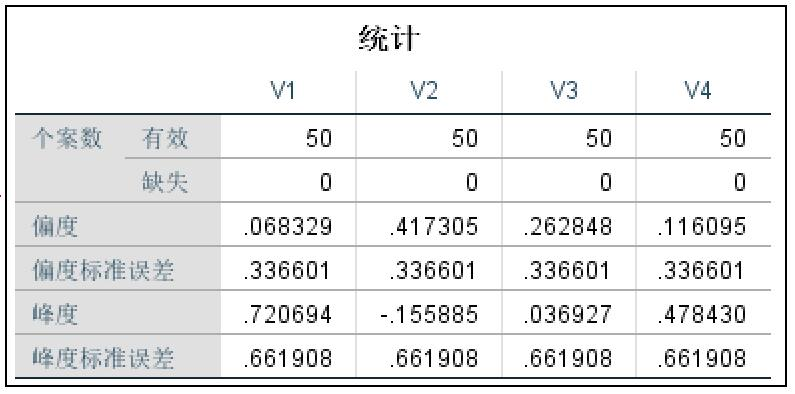
\includegraphics[scale=0.5]{1_piandu.jpg}
				\caption{偏度与峰度}
			\end{figure}
			\qquad 由图中数据计算可得可得Z-Scroe均处于±1.96之间,可认为四组数据均服从正态分布。			
		\end{enumerate}
		\item 图形判断
		
		1.直方图:表示连续性变量的频数分布,可以用来考察是否服从正态分布
		
		\qquad 通过SPSS处理部分数据得到的结果如下图:
		\begin{figure}[H]
			\centering %图片居中显示
			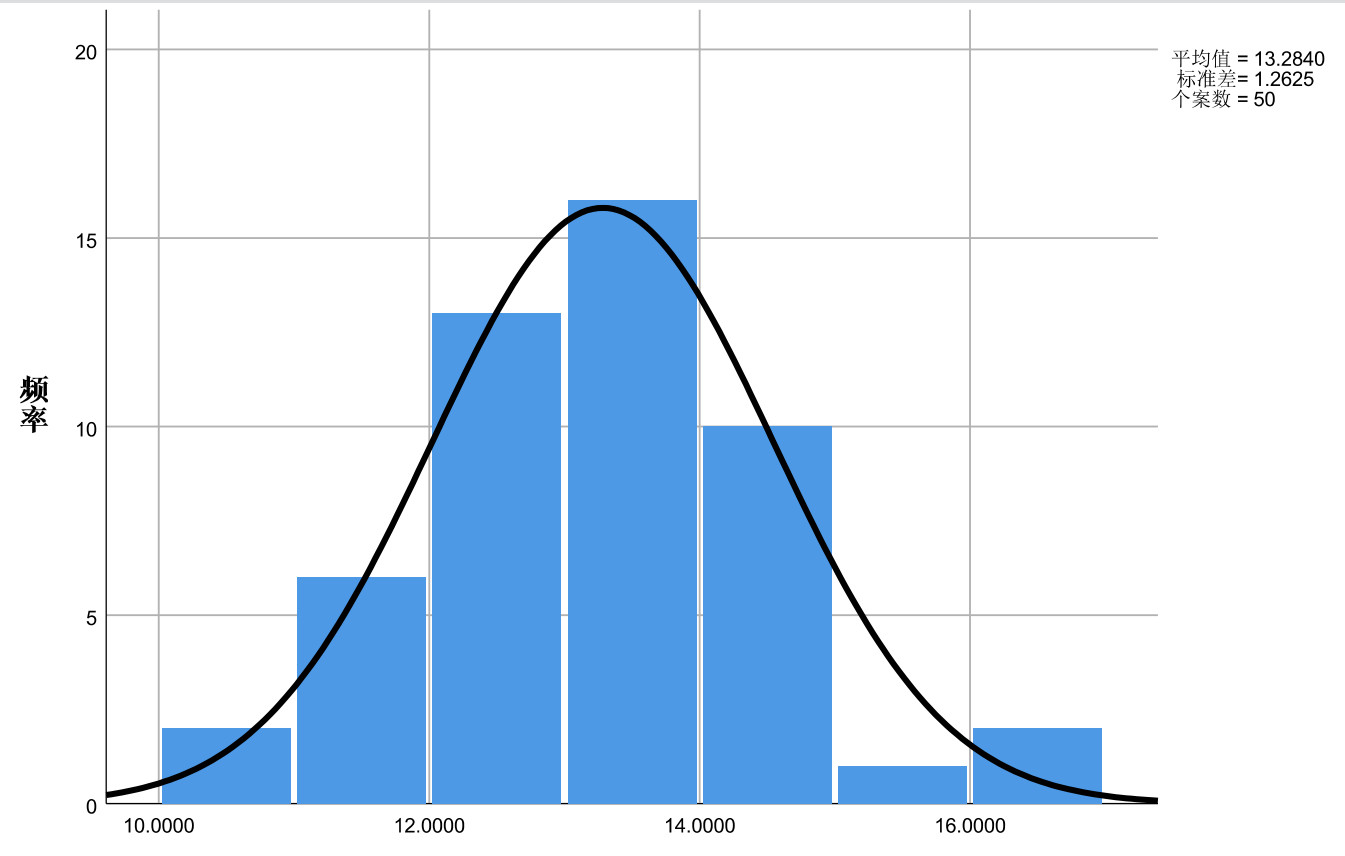
\includegraphics[scale=0.5]{1_zhifang.jpg}
			\caption{直方图}
		\end{figure}
		2.P-P图和Q-Q图
		
		\qquad P-P图反映了变量的实际累积概率与理论累积概率的符合程度,Q-Q图反映了变量的实际分布与理论分布的符合程度。若数据点与理论直线(即对角线)基本重合,就认为数据服从正态分布。
		
		\qquad 通过SPSS处理部分数据得到的结果如下图:
		
		\begin{figure}[H]
			\centering
			\subfigure[P-P图]{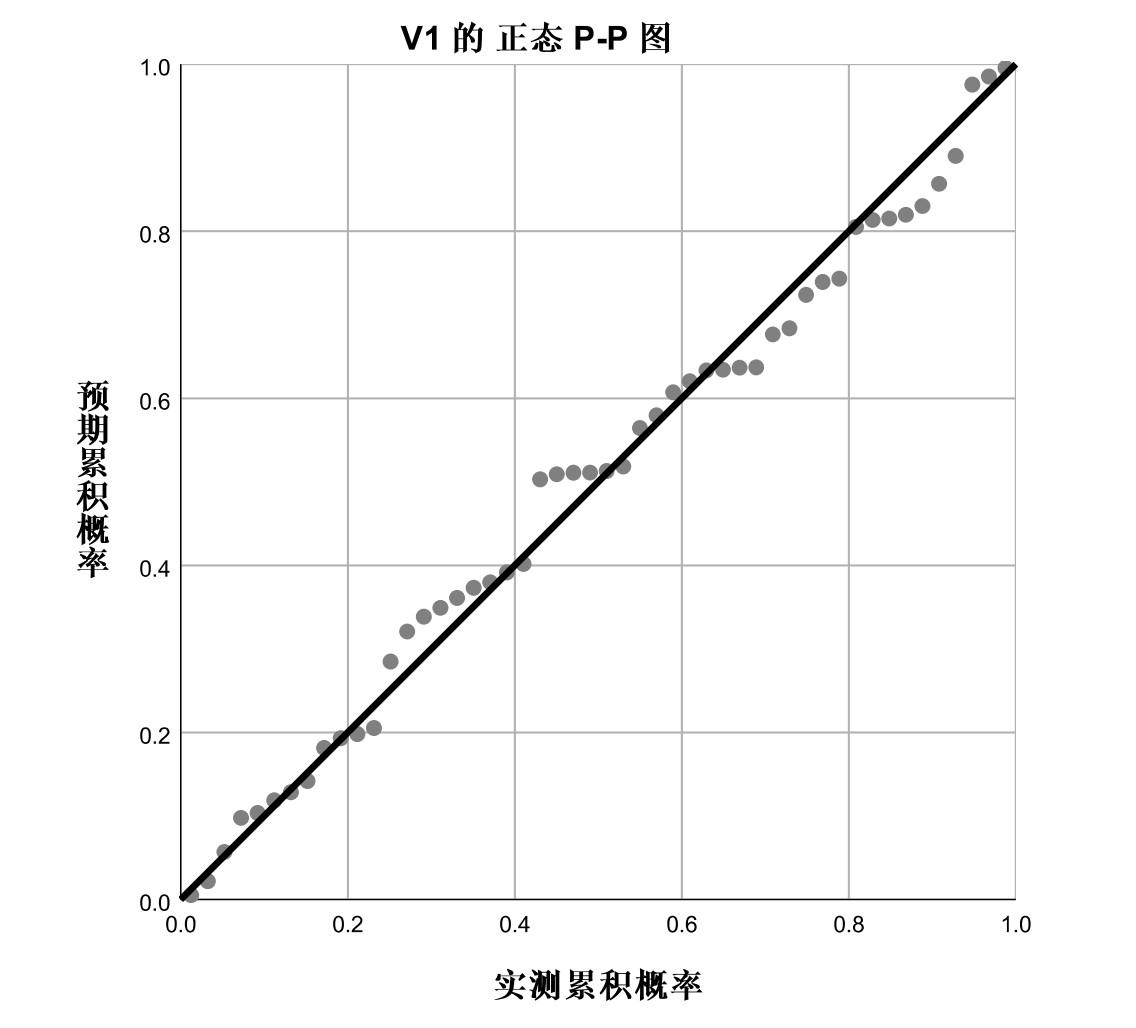
\includegraphics[scale=0.5]{1_pp.jpg}}
			\subfigure[Q-Q图]{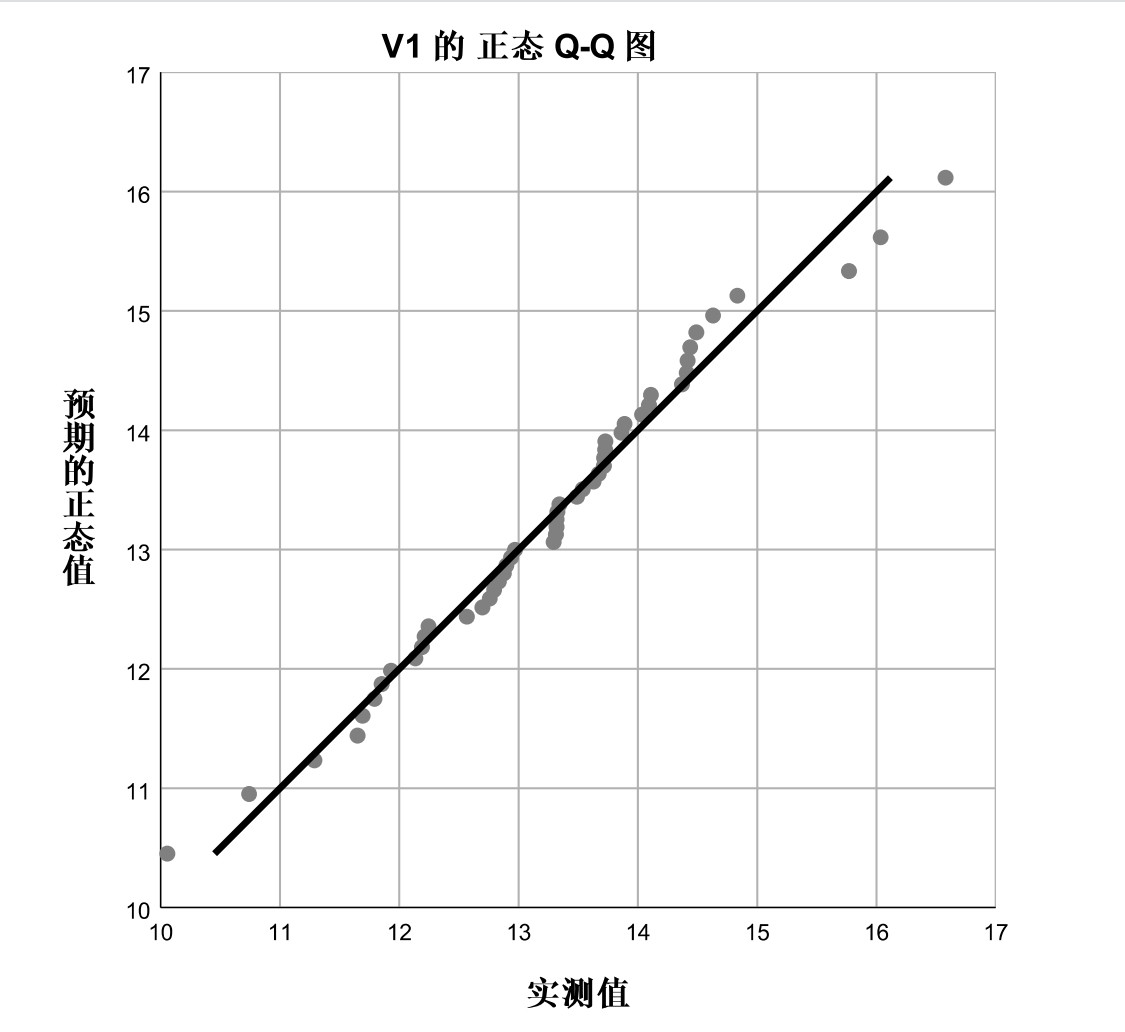
\includegraphics[scale=0.5]{1_qq.jpg}}
			\caption{ P-P图和Q-Q图 }
		\end{figure}
		
		\qquad 由图可知P-P图和Q-Q图的数据点都与应与对角线基本重合,所以认为数据符合正态分布。
	\end{itemize}
	\subsubsection{统计分析}
	经过上述对部分数据的正态性检验,我们可以认为附件1中每组数据均服从正态分布。统计分析中的概率分布均采用正态分布进行处理。
	
	1.数据预处理 
	
	使用EXCEL对数据进行对数据进行分列处理和简单的数据清洗,将数据以矩阵形式输入MATLAB。矩阵每行数据为某类疫苗在某个工位模拟处加工50次的生产时间。
	
	2. 用MATLAB进行统计分析
	
	在MATLAB中使用求平均数、方差、最值的函数对输入数据的矩阵逐行处理并储存,结果如表2-5显示,结果定量地体现了每个工位对10种疫苗不同的生产水平,对疫苗生产具有重要参考价值。
\begin{table}[!ht]
		\caption{工位CJ1的疫苗生产水平}\label{1tou}
		\begin{tabular*}{\hsize}{@{}@{\extracolsep{\fill}}c|c|c|c|c|c|c|c|c|c|c }
			\toprule[2pt]
			& YM1 & 	YM2 & 	YM3 & 	YM4 & 	YM5 & 	YM6 & 	YM7 & 	YM8 & 	YM9 & 	YM10  \\
			\hline
			均值  &   13.284   &   9.870  & 	20.058  & 	7.988  & 	8.770  & 	 19.074  & 	11.160  & 	16.020  & 	15.014 & 	12.952 \\
			
			方差  &    1.593  &	0.833   &	0.844   &	0.932  &	0.745  &	1.334    &	1.026       &	1.131   &	0.973  &	0.207    \\
			
			最小值&10.055&	6.970&	17.814&	5.872&	5.927&	16.435&	8.843&	13.575&	12.823&	11.463\\
			
			最大值&16.578&	11.682&	21.814&	10.038&	10.384&	21.752&	13.287&	18.078&	17.412&	13.618\\
			\bottomrule[2pt]			
		\end{tabular*}
	\end{table}
	\begin{table}[!ht]
		\caption{工位CJ2的疫苗生产水平}\label{}
		\begin{tabular*}{\hsize}{@{}@{\extracolsep{\fill}}c|c|c|c|c|c|c|c|c|c|c }
			\toprule[2pt]
			& YM1 & 	YM2 & 	YM3 & 	YM4 & 	YM5 & 	YM6 & 	YM7 & 	YM8 & 	YM9 & 	YM10  \\
			\hline
			均值  &   14.962  &   19.907    & 	15.972  & 9.936	  & 	13.722  & 	20.094   & 	16.496  & 	8.827  & 12.035	 & 7.011	 \\
			
			方差  &   1.0830   &	1.252    &	0.693   &	0.953    &	1.139       &	0.973    &	0.929       &	0.261  &	1.158   &	0.282   \\
			
			最小值&13.067&	17.513&	13.978&	7.640&	11.796&	17.500&	14.680&	7.967&	10.093&	5.950\\
			
			最大值&17.585&	22.229&	17.809&	12.508&	16.605&	21.927&	18.730&	10.187&	14.748&	8.579\\
			\bottomrule[2pt]			
		\end{tabular*}
	\end{table}
	\begin{table}[!ht]
		\caption{工位CJ3的疫苗生产水平}\label{}
		\begin{tabular*}{\hsize}{@{}@{\extracolsep{\fill}}c|c|c|c|c|c|c|c|c|c|c }
			\toprule[2pt]
			& YM1 & 	YM2 & 	YM3 & 	YM4 & 	YM5 & 	YM6 & 	YM7 & 	YM8 & 	YM9 & 	YM10  \\
			\hline
			均值  &   19.846   &   17.928    & 	14.970  & 	5.935  & 	13.005  & 	 14.148  & 	12.013  & 	18.114  & 7.041	 & 	9.049 \\
			
			方差  &   1.187    &	0.902	   &	1.040   &	0.037 &	0.831   &	0.875    &	0.786       &	1.070   &	0.133   &	0.207 \\
			
			最小值& 17.861&	15.503&	12.671&	5.3536&	10.798&	12.090&	9.652&	16.315&	6.231&	7.974 \\
			
			最大值&22.908&	20.177&	17.787&	6.3889&	15.010&	15.813&	14.436&	21.569&	7.994&	9.817\\
			\bottomrule[2pt]			
		\end{tabular*}
	\end{table}
	\begin{table}[!ht]
		\caption{工位CJ4的疫苗生产水平}\label{1wei}
		\begin{tabular*}{\hsize}{@{}@{\extracolsep{\fill}}c|c|c|c|c|c|c|c|c|c|c }
			\toprule[2pt]
			& YM1 & 	YM2 & 	YM3 & 	YM4 & 	YM5 & 	YM6 & 	YM7 & 	YM8 & 	YM9 & 	YM10  \\
			\hline
			均值  &   20.012   &   18.942    & 	15.116  & 	18.128  & 	11.249  & 	 13.883  & 	19.087  & 	16.831  & 8.949	 & 	16.052 \\
			
			方差  &  1.889     &	0.890     &	0.812   &	1.127   &	1.230   &	1.151   &	0.656       &	0.912   &	0.175   &	0.263 \\
			
			最小值& 16.505&	17.164&	12.806&	16.043&	9.231&	11.724&	16.740&	14.747&	8.108&	14.950 \\
			
			最大值&23.789&	21.424&	17.003&	20.789&	14.526&	16.949&	20.755&	18.735&	9.898&	17.487\\
			\bottomrule[2pt]			
		\end{tabular*}
	\end{table}
	
	对于概率分析,经正态性检验可知,数据服从正态分布,由均值和方差我们可以画出每组数据的正态分布曲线,近似于数据本身的概率分布曲线。结果如图显示。从概率分布曲线我们可以更宏观且直观地了解每个工位生产疫苗的能力水平。
	
	\begin{figure}[H]
		\centering %图片居中显示
		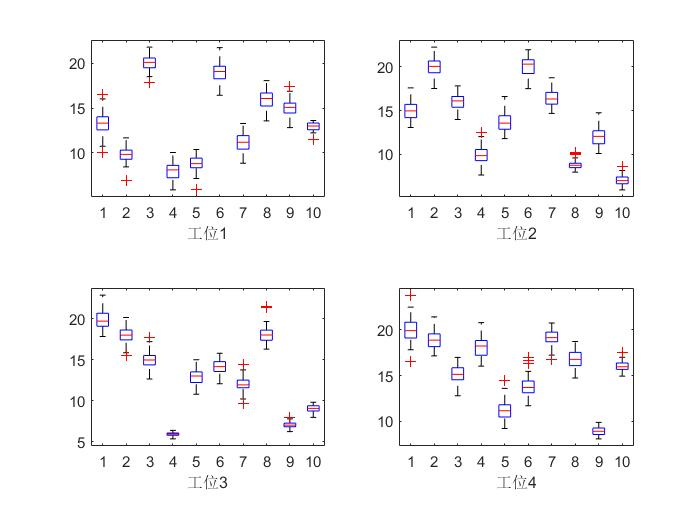
\includegraphics[scale=0.5]{箱型图new.jpg}
		\caption{四个工位生产每种疫苗用时分布的箱型图}
	\end{figure}
	在统计分析中,我们采用数据表格和曲线图像两种方式,定性和定量地全面分析了不同工位对不同疫苗的生产能力水平,有利于直观明了地掌握掌握工位生产疫苗的能力水平,为疫苗生产提供参考。
	
	\subsection{问题二}
	\subsubsection{生产过程分析}
	根据题意,绘制出生产过程的示意图如下图\ref{pipeline1}所示。CJ1$\sim$CJ4表示4个工位,从左往右表示时间流逝的过程,各个颜色的区块表示不同种疫苗的生产时间段。
	\begin{figure}[H]
		\centering %图片居中显示
		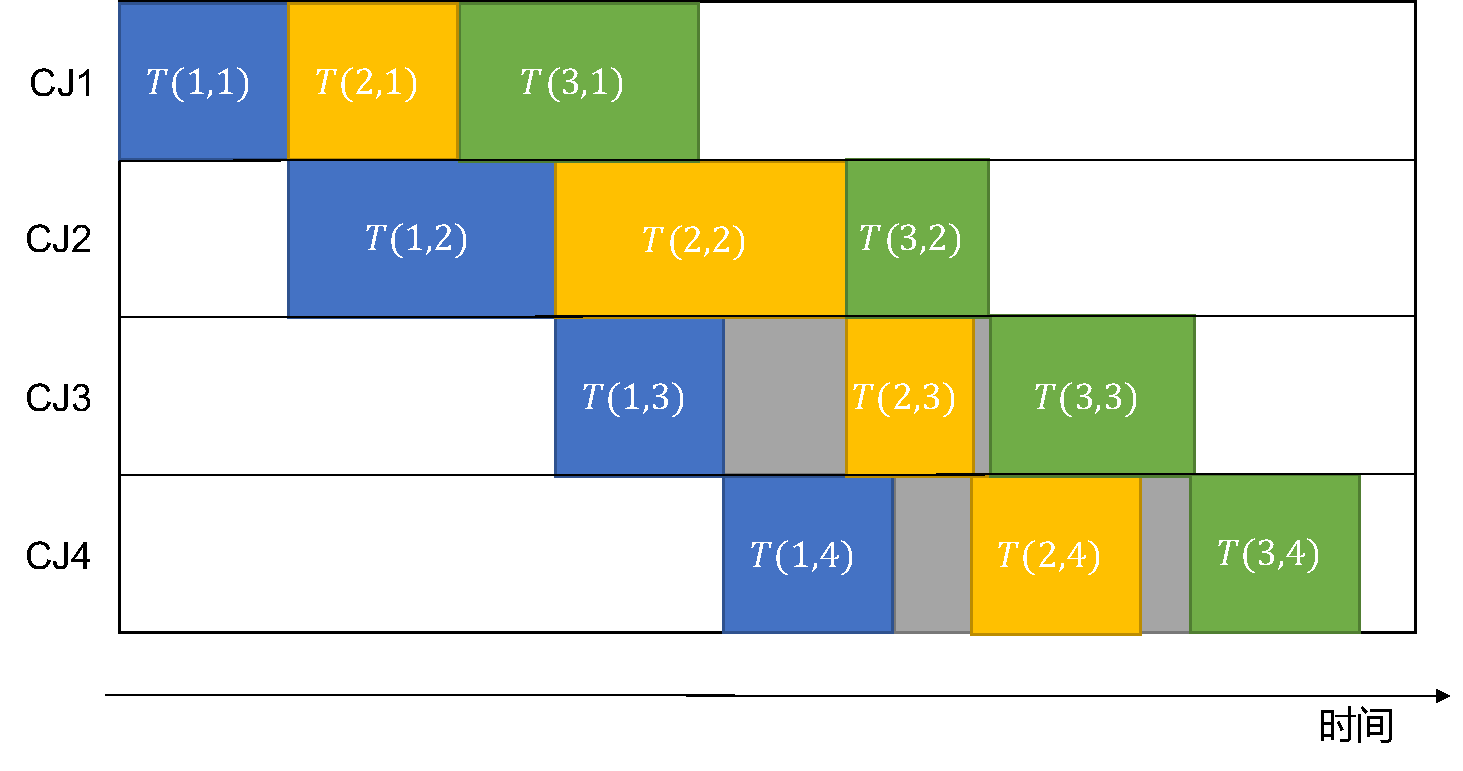
\includegraphics[scale=0.5]{pipe1.pdf}
		\caption{生产过程示意图}\label{pipeline1}
	\end{figure}
	由图\ref{pipeline1}可知,后续工位在生产过程中,由于下一疫苗还未完成在前一工位的生产,因此会有等待时间$T_{W}$(灰色区块)。用$\Omega_{in}(k,j)$、$\Omega_{out}(k,j)$分别表示顺序第$k$位的疫苗进入和退出工位CJ$j$的时刻。则总时间$T_{\Sigma}$可以表示为$T_{\Sigma}。(\boldsymbol{x})=\Omega_{out}(10,4)-\Omega_{in}(1,1)$
	\subsubsection{模型建立}
%	从整体来看,本题所有问题属于流水线平衡和优化问题,均可分为优化算法和平衡目标两大方面。%基于 0 - 1 规划的成衣制造流水线平衡建模与仿真
%	平衡目标即我们规范设置的满足约束条件的目标函数,属于模型建立,而优化算法则是我们求解目标函数的算法,是模型求解的主要内容。
%		
%	问题二中目标函数易于表示,但约束条件为非线性无法脱离目标函数单独计算。所以我们采用MATLAB构建求解总时间函数,总时间的求解算法采用流水线算法,该算法基于流水线平衡理论,结合具体约束条件。
	
	建立优化模型确定约束条件:
	\begin{itemize}
		\item 决策变量 
		\par 本问题的决策变量$\boldsymbol{x}=(x_{1},x_{2},\dots,x_{10})$表示10种疫苗的生产顺序排列,其中一个元素$x_{k}$表示第$k$个被生产的疫苗,其值$x_{k}\in$(YM1,YM2,$\dots$,YM10)。
		\item 目标函数
		\par 本问题的目标是使得总时间$T_{\Sigma}$最小,由图\ref{pipeline1}可知,总时间可用最后一个疫苗离开工位4的时刻与第一个疫苗进入工位1作差求得。因而目标函数可表示为
		\begin{equation}
			\min \quad T_{\Sigma}(\boldsymbol{x})=\Omega_{out}(10,4)-\Omega_{in}(1,1)
		\end{equation}
		\item 约束条件
		\par 前一种类型的疫苗离开某个工位后,后一种类型的疫苗才能进入这个工位。即后一疫苗进入此工位的时刻应大于前一疫苗离开的时刻。即
	\begin{equation}
		\Omega_{in}(k,j)\geqslant\Omega_{out}(k-1,j)
	\end{equation}
	当前疫苗须在离开上一工位后才能进入下一工位,即
	\begin{equation}
		\Omega_{in}(k,j)\geqslant\Omega_{out}(k,j-1)
	\end{equation}
	疫苗在一个工位上生产完才可离开,即
	\begin{equation}
		\Omega_{out}(k,j)\geqslant\Omega_{in}(k,j)+t(k,j)
	\end{equation}
	设第一个疫苗进入第一个工位的时刻为0,即
	\begin{equation}
		\Omega_{in}(1,1)=0
		\label{eq0}
	\end{equation}

	不考虑每个疫苗在每个工位上生产耗时的随机性,可以确定其值为平均值,即
	\begin{equation}
		t(k,j)=\mu(x_{k},j)
		\label{eq1}
	\end{equation}
		


	\item 总体模型
	\par 总体的优化模型如下:
	\begin{equation}
		\begin{split}
		\min \quad&T_{\Sigma}(\boldsymbol{x})=\Omega_{out}(10,4)-\Omega_{in}(1,1)\\
		s.t. \quad &\Omega_{in}(k,j)\geqslant\Omega_{out}(k-1,j)\\
		&\Omega_{in}(k,j)\geqslant\Omega_{out}(k,j-1)\\
		&\Omega_{out}(k,j)\geqslant\Omega_{in}(k,j)+t(k,j)\\
		&\Omega_{in}(1,1)=0\\
		&t(k,j)=\mu(x_{k},j)
		\end{split}
	\end{equation}

	\end{itemize}

%	从图可以看出,总时间可以用工位CJ4的总时间计算,即工位CJ4的生产时间加其等待时间。而工位CJ4的等待时间又和工位CJ3的生产时间和等待时间有关。如此,问题由通过循环和判断构成。我们结合求每个工位当前总时间的循环语句和疫苗进入每个工位时前后工位总时间的大小的判断语句,构造出符合题意的function[t]。
	
	\subsubsection{模型求解}
	若要使得总时间最小,需要让$\Omega_{in}(i,j)$和$\Omega_{out}(i,j)$取其取值区间最左端的值。因而可得到如下递推关系:
	\begin{equation}
		\Omega_{out}(k,j)=\Omega_{in}(k,j)+t(k,j)
		\label{eq7}
	\end{equation}
	\begin{equation}
		\Omega_{in}(k,j)=\max\{\Omega_{out}(k-1,j),\Omega_{out}(k,j-1)\}
		\label{eq8}
	\end{equation}
	从而,总时间$T_{\Sigma}$可以依据式\ref{eq7}、式\ref{eq8}运用递归算法求得。结合式\ref{eq0}、\ref{eq1},可以推断出,$T_{\Sigma}$是$t(k,j)$的线性组合,也是$\mu(i,j)$的线性组合。即给定生产顺序$\boldsymbol{x}$,设$x_{k}=$YM$i$,可确定
	\begin{equation}
	\begin{split}
		T_{\Sigma}&=\sum_{k,j}\alpha(x_{k},j)t(k,j)\\
		&=\sum_{i,j}\alpha(i,j)\mu(i,j)
		\label{linear}
	\end{split}
	\end{equation}
	$\alpha(i,j)$的值随着生产顺序的不同而不同,从而改变总时间。由于$\alpha(i,j)$与顺序的关系是非线性的,因此本题目标函数仍为非线性。
	\par 对于这样一个非线性优化问题,需要在解空间搜索最优解。本题若采取暴力求解算法,需要遍历10!个解得到对应的总时间再比较,不具有实际性和通用性。因此需要使用算法减少遍历次数。
	本问题属于非线性最优化问题,其目标函数难以显式表达,因此采用启发式算法求近似最优解。这里我们选用模拟退火算法。 
	\par 模拟退火算法是一种通用概率启发式算法,用来在一个大的搜寻空间内寻找问 题的最优解。本问题的目标是求出饲料质量即总亲缘度最高的原料混合分配方案。 模拟退火算法具有高效、鲁棒、通用、灵活的优点,因而利用模拟退火可以避免在 求解过程中陷入局部最优。
	本题模拟退火算法的步骤:
	\begin{enumerate}
		\item 解空间和初始解:算法的每一个解为十种类型疫苗的不同排列
		\begin{equation}
		S=\{(x_1,x_2,\dots,x_{10})|x_{i}\in[YM1,YM2,\dots,YM10],x_{i}\neq x_{j}\}
		\end{equation}
		其中$x_{i}$表示第$i$个被生产的疫苗编号。
						
		\qquad 本模型中初始解为随机生成的生产顺序序列$S_{0}$。$S_{0}$经验证满足所有约束条件。

		\item 目标函数:
		\begin{equation*}
		f = \min T_{\Sigma}
		\end{equation*}
		
		\item 邻解生成:
		
		\qquad 邻解为不同于当前的生产顺序序列,本题中采取对当前序列进行随机性简单变换。70\%可能随机将序列中的两个疫苗生产顺序互换,30\%对三个生产顺序互换。
		
		\item 目标函数差值降温接收准则:
		
		\qquad 新解产生,经过目标函数得到新的总时间$ T_{new} $
		
		\qquad 如果$ \Delta t = T_{new} - T_{0}  \textless 0 $ ,则接受 $   T_{new}$ 作为新的当前解 $ T_{now} $
		
		\qquad 否则以概率 $exp \left( -\Delta t/ T\right)$接受 $   T_{new}$ 作为新的当前解 $ T_{now} $。
		
		\item 降温:
		
		\qquad 利用选定的降温系数$\alpha$进行降温,每次解更新降温一次:
		\begin{equation*}
		T \gets \alpha
		\end{equation*}
				
		\item 参数设定:
		
		\qquad 我们设定初始温度
		\begin{equation*}
		T_{0} = 120
		\end{equation*}
		
		\qquad 最终温度
		\begin{equation*}
		T_{f} = 1
		\end{equation*}
		
		\qquad 温度衰减系数$ \alpha = 0.99 $,即:
		\begin{equation*}
		 T^{'} = 0.99 T
		\end{equation*}
			
		\qquad Markov马尔科夫链长度
		\begin{equation*}
		L_{Markov} = 10000
		\end{equation*}
		
		\qquad 用 MATLAB编写模拟退火算法对问题进行求解,得到以下进化曲线:
		\begin{figure}[H]
			\centering %图片居中显示
			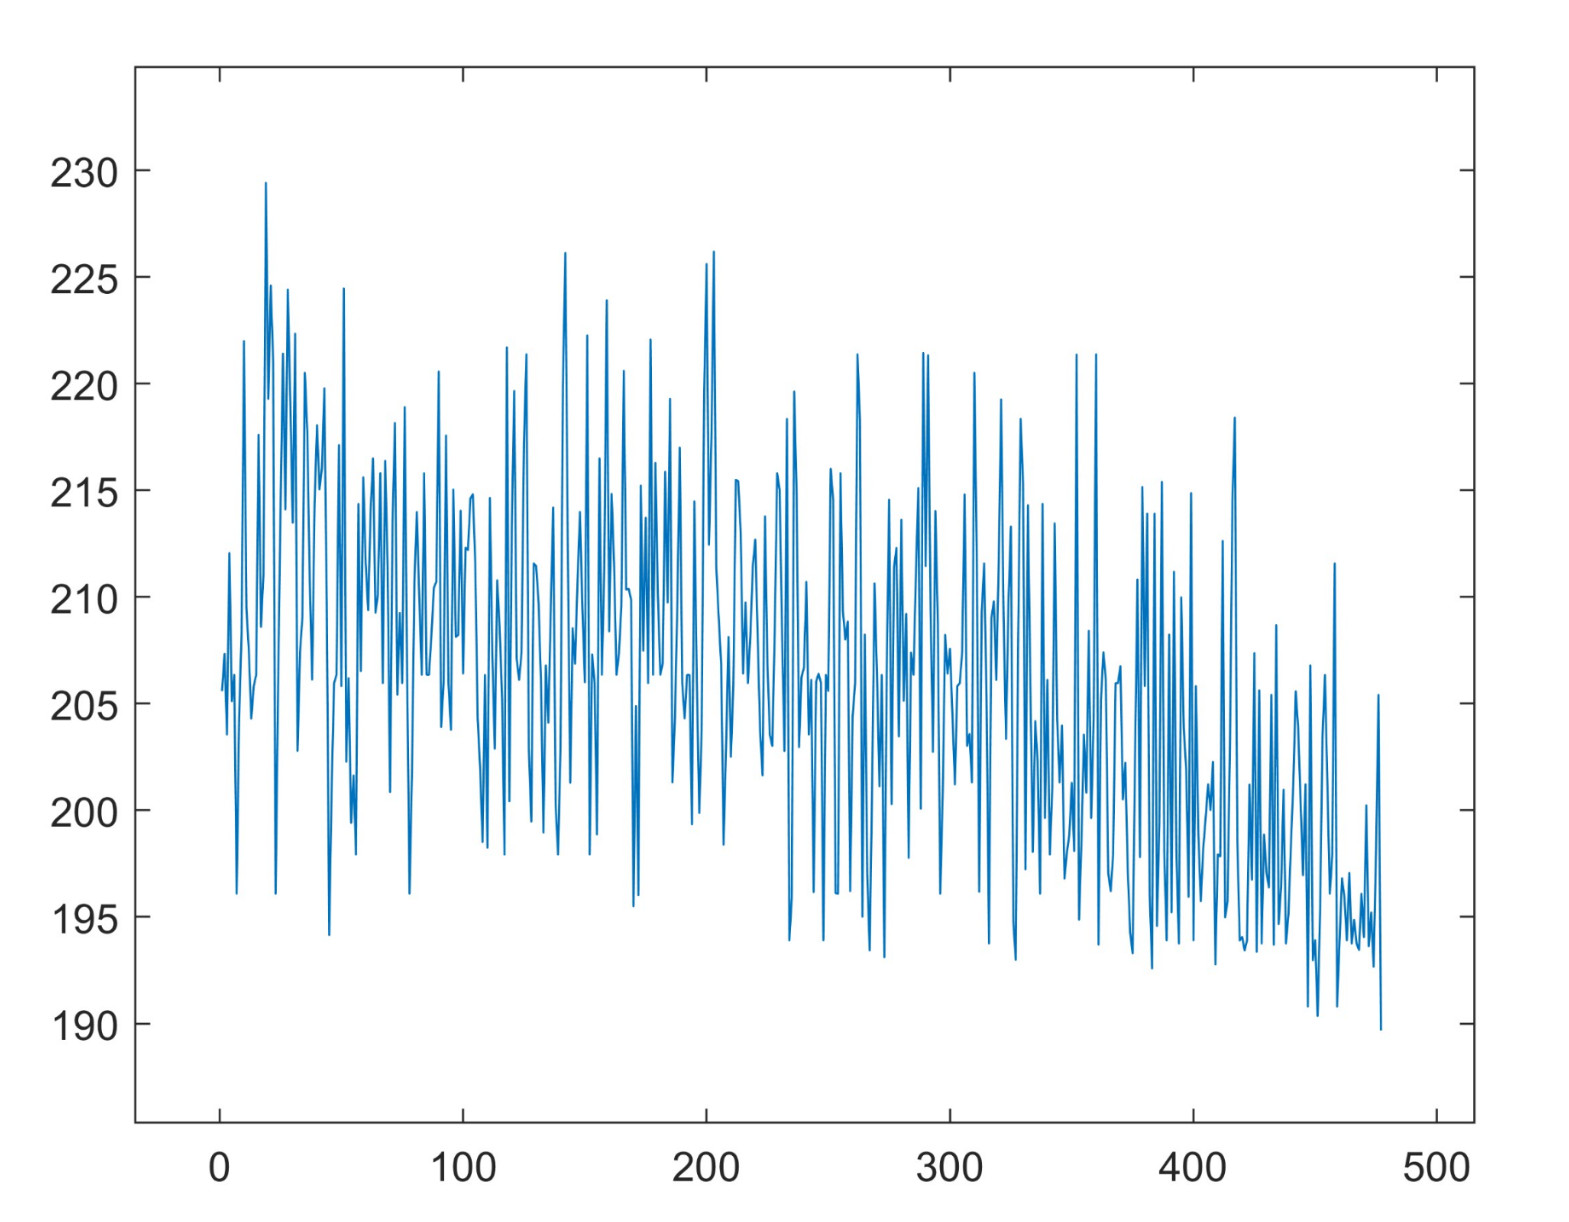
\includegraphics[scale=0.5]{2_moni.jpg}
			\caption{模拟退火算法目标函数迭代曲线}
		\end{figure}

	最终得出最优解,生产总时间为$ T_{\min} = 187.8657 $
	
	相对应的疫苗生产顺序如表所示:
	\begin{table}[H]
		\centering
		\caption{问题2的结果}
		\begin{tabular}{ c| c| c }
			\hline
			加工顺序(填疫苗编号) & 进入CJ1时刻 & 离开CJ4时刻 \\
			\hline
			 4 & 00:00 & 00:48 \\
			 \hline
			 10 & 00:08 & 01:04 \\
			 \hline
			 5 & 00:21 & 01:15 \\
			 \hline
			 7 &  00:30 & 01:34\\
			 \hline
			 8 & 00:41 & 01:51\\
			 \hline
			 1 &  00:57 & 02:11\\
			 \hline
			 3 & 01:10 & 02:26\\
			 \hline
			 2 & 01:30 & 02:45\\
			 \hline
			 9 &  01:40 & 02:54\\
			 \hline
			 6 & 01:55 & 03:08 \\
			\hline
		\end{tabular}
	\end{table}

	色块图
		\begin{figure}[H]
			\centering %图片居中显示
			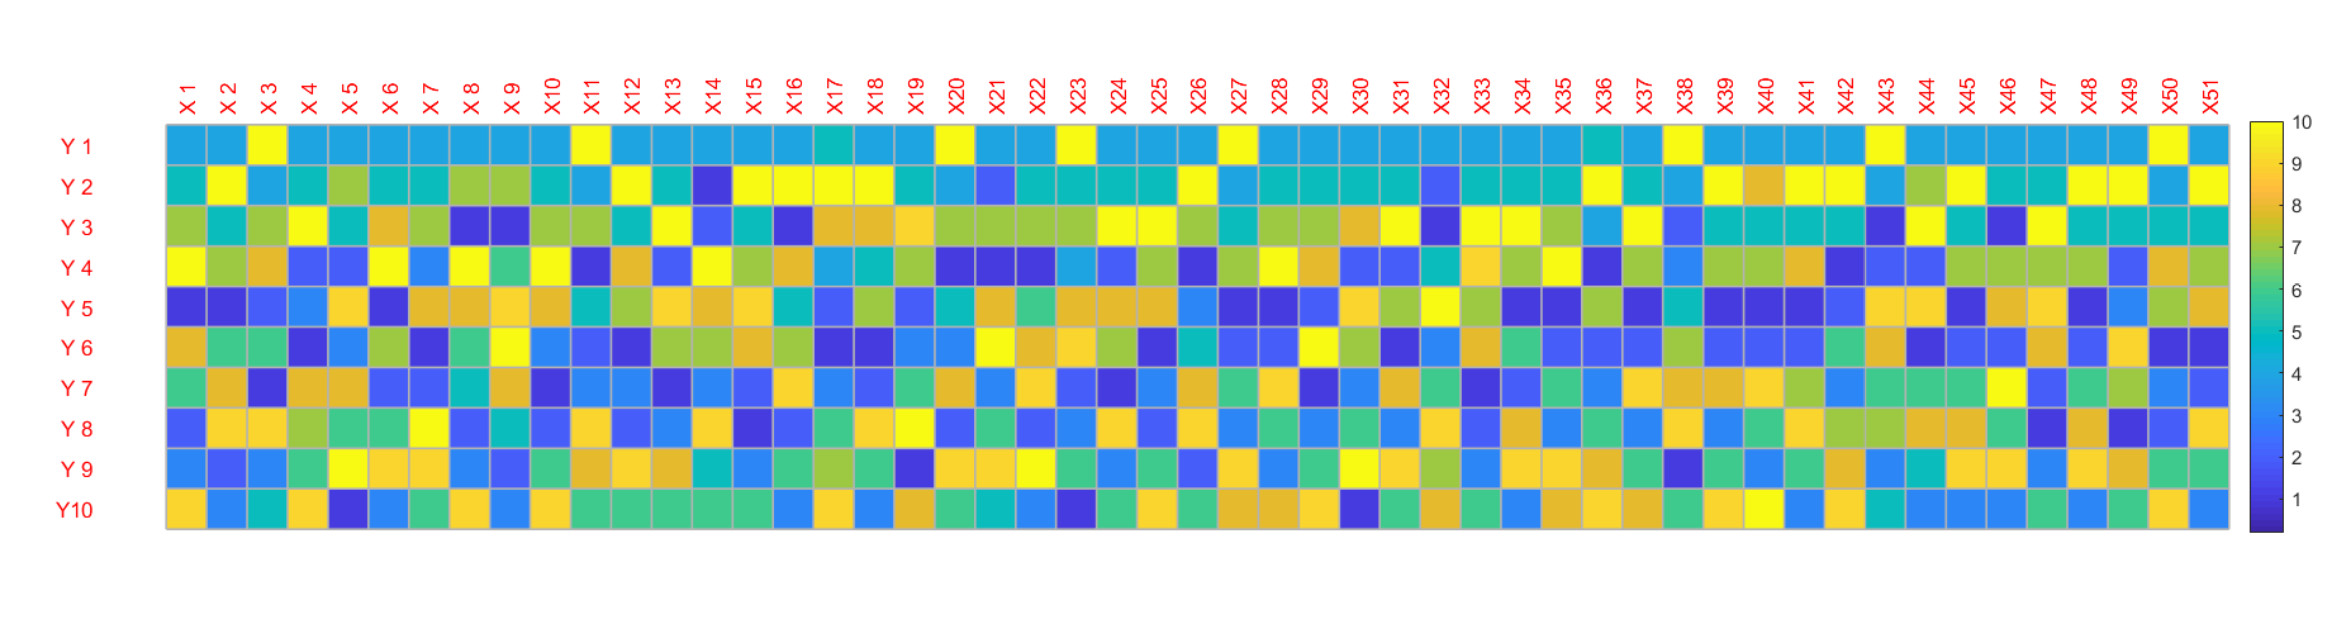
\includegraphics[scale=0.5]{2_sekuai.jpg}
			\caption{色块图}
		\end{figure}
	\end{enumerate}
	
	\subsubsection{模型分析}
	
	\subsection{问题三}
	\subsubsection{模型建立}
	与问题二相比,需要改变目标函数并考虑随机性。
	\par 考虑生产用时的随机性,每个工位生产每种疫苗的所需时间$T(i,j)$均符合正态分布,即
	\begin{equation}
	T(i,j)\sim\mathcal{N}(\mu(i,j),\sigma^2(i,j))
	\end{equation}
	%插入图,流水线
	\par 由式\ref{linear}可知,总用时是$t(k,j)$的线性组合。由于
	\begin{equation}
	t(k,j)=T(x_{k},j)\sim\mathcal{N}(\mu(x_{k},j),\sigma^2(x_{k},j))
	\end{equation}
	结合定理1,可知总用时$T_{\Sigma}$也符合正态分布。即
	\begin{equation}
	T_{\Sigma}\sim\mathcal{N}(\mu_{\Sigma},\sigma_{\Sigma})
	\end{equation}
	由定理2,可以求出其正态分布的参数
	\begin{equation}
		\mu_{\Sigma}=\sum_{i,j}\alpha(i,j)\mu(i,j),\sigma_{\Sigma}^{2}=\sum_{i,j}\alpha(i,j)\sigma^{2}(i,j)
		\label{all}
	\end{equation}
	\par 设问题2求出的最短时间为$T_{\min}$,本问题的目标是使得$T_{\Sigma}<0.95T_{\min}$的概率最大。可以用概率分布函数求出。
	\begin{equation}
        	\begin{split}
        	\max P(T_{\Sigma}<0.95T_{\min})&=F_{\Sigma}(x)|_{x=0.95T_{\min}}\\
			&=\frac{1}{\sqrt{2\pi}\sigma_{\Sigma}}\int^{x}_{-\infty}\exp[{-\frac{(t-\mu_{\Sigma})^2}{2\sigma_{\Sigma}^2}}]dt\arrowvert_{x=0.95T_{\min}}
        	\end{split}
		\label{pr}
	\end{equation}

	\subsubsection{模型求解}
	在问题二中,由于生产耗时固定,因而在生产顺序也确定的情况下,$T_{\Sigma}$表达式中的系数$\alpha(i,j)$都可确定。而本题虽然每个工位生产每种疫苗的耗时有随机性,但是其大小对比关系基本不变。因此也可以认为在生产顺序固定的情况下其系数$\alpha(i,j)$均确定。
	改变评价函数为概率值,用模拟退火算法求解。得到使概率最大的生产的最优顺序为
	\begin{equation}
		\boldsymbol{x}^{*}=(YM4,YM10,YM7,YM8,YM2,YM9,YM1,YM5,YM3,YM6)
	\end{equation}
	总时间可以表示为
	\begin{equation}
		T_{\Sigma}=T(1,1)+T(1,2)+T(1,3)+\sum_{i}^{10}T(i,4)
	\end{equation}
	由式\ref{all},可以求总时间正态分布的参数为
	\begin{equation}
		\mu_{\Sigma}=185,\sigma_{\Sigma}^{2}=(3.728)^2
	\end{equation}
	再由式\ref{pr},可以求得最大概率为$P_{\max}=24.79\%$,
	\par 在确定生产顺序的情况下,缩短的时间比例$\delta$与最大概率之间的关系为
	\begin{equation}
	\begin{split}
		P_{\max}=f(\delta)=\frac{1}{\sqrt{2\pi}\cdot3.728}\int^{(1-\delta)T_{\min}}_{-\infty}\exp[{-\frac{(t-185)^2}{2\cdot(3.728)^2}}]dt
	\end{split}
	\end{equation}
	
	\subsection{问题四}
	\subsubsection{模型描述与假设}
	本题中,约束条件增加为每种类型疫苗的生产任务不可拆分和在可靠性为90\%的前提下。所以为了简便求解,我们这一题的重点不在细节地通过生产顺序来计算流水线平衡目标。而是通过整体流水线的正态分布特性使用概率和微分方程进行求解。
	
	另外,为了方便求解。我们不采用多个独立事件的概率乘法公式作为目标函数,即不以每天每工位生产的可靠性作为独立事件,使乘法公式结果为90\%的概率。而是通过整体求解再可靠性90\%前提下的最大总时间。
	\subsubsection{模型建立}
	由流水线图\ref{pipeline2}可知,其每天生产时间由耗时最多的工位决定。
	\begin{figure}[H]
		\centering %图片居中显示
		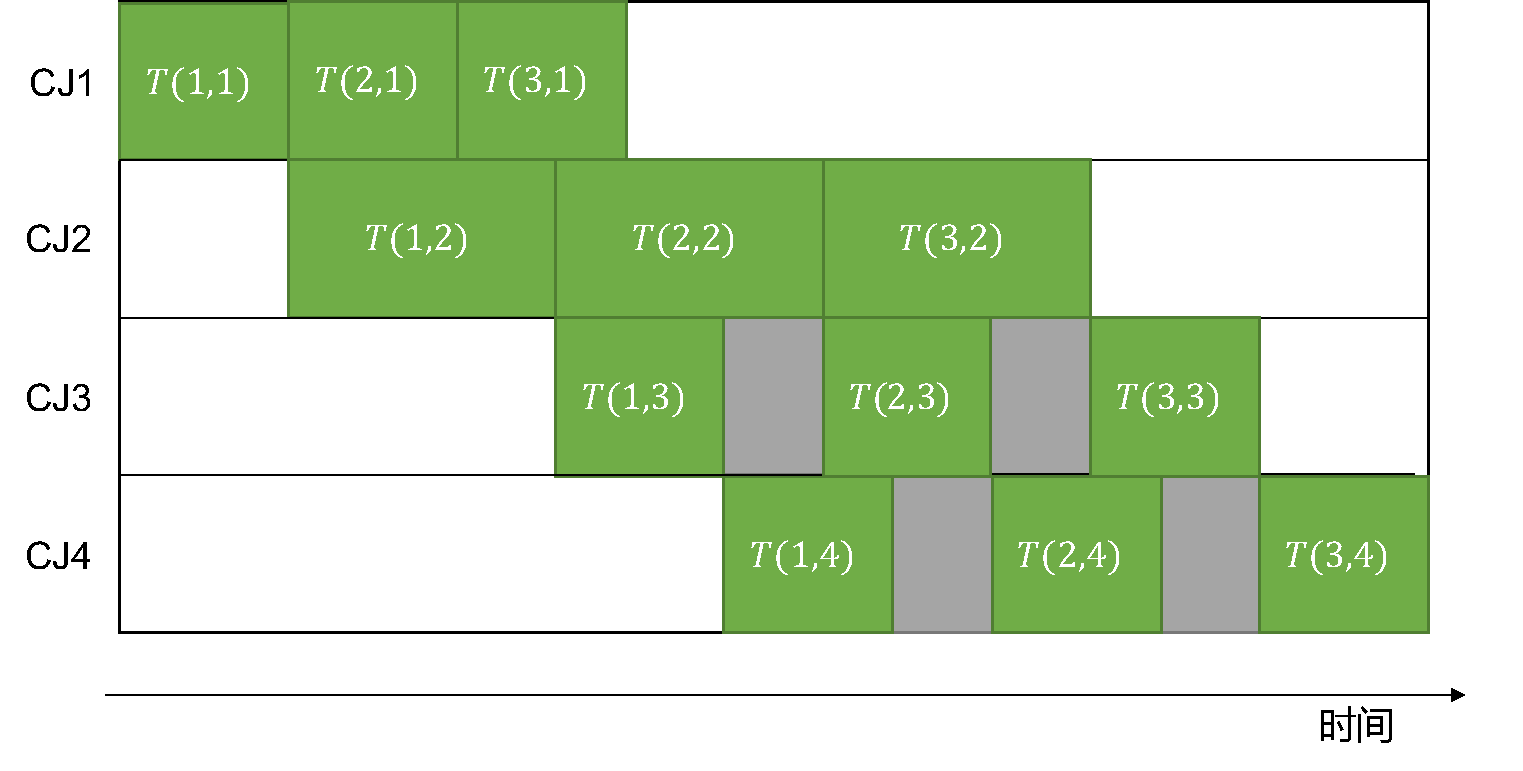
\includegraphics[scale=0.5]{pipe2.pdf}
		\caption{生产过程示意图}\label{pipeline2}
	\end{figure}
	由于每类疫苗的生产不可拆分,因此不需要考虑其生产顺序,在一定时间内流水线上仅生产同一类疫苗。则一天生产时间$t$服从正态分布,$t\sim\mathcal{N}(\mu,\sigma^2)$。
	
	由正态分布的定理2可知,多个独立正态分布的线性组合仍然服从正态分布。
	
	总时间可以看$X$天最大耗时的线性组合,因此最终的总时间也服从正态分布。我们求出此正态分布的参数。我们假定总共经过$N$整天完成生产,则总时间$X$可以看成$Nt$,$Nt$服从正态分布,$Nt\sim\mathcal{N}(N\mu,N\sigma^2)$。
	
	因此总时间$X$的分布函数可以表示为
	\begin{equation}
	F(x)=\frac{1}{\sqrt{2\pi}N\sigma}\int^{x}_{-\infty}e^{-\frac{t-N\mu)^2}{2N^2\sigma^2}}dt
	\end{equation}
	为从整体满足可靠性90\%,我们需要求以下解积分方程:
	\begin{equation}
	\frac{1}{\sqrt{2\pi}N\sigma}\int^{x}_{-\infty}e^{-\frac{(t-N\mu)^2}{2N^2\sigma^2}}dt = 0.9
	\end{equation}
	该积分方程的解析解为满足可靠性要求的最短时间。
	\subsubsection{模型求解}
	求出总时间$Nt$的概率分布函数如图所示:
	\begin{figure}[H]
		\centering %图片居中显示
		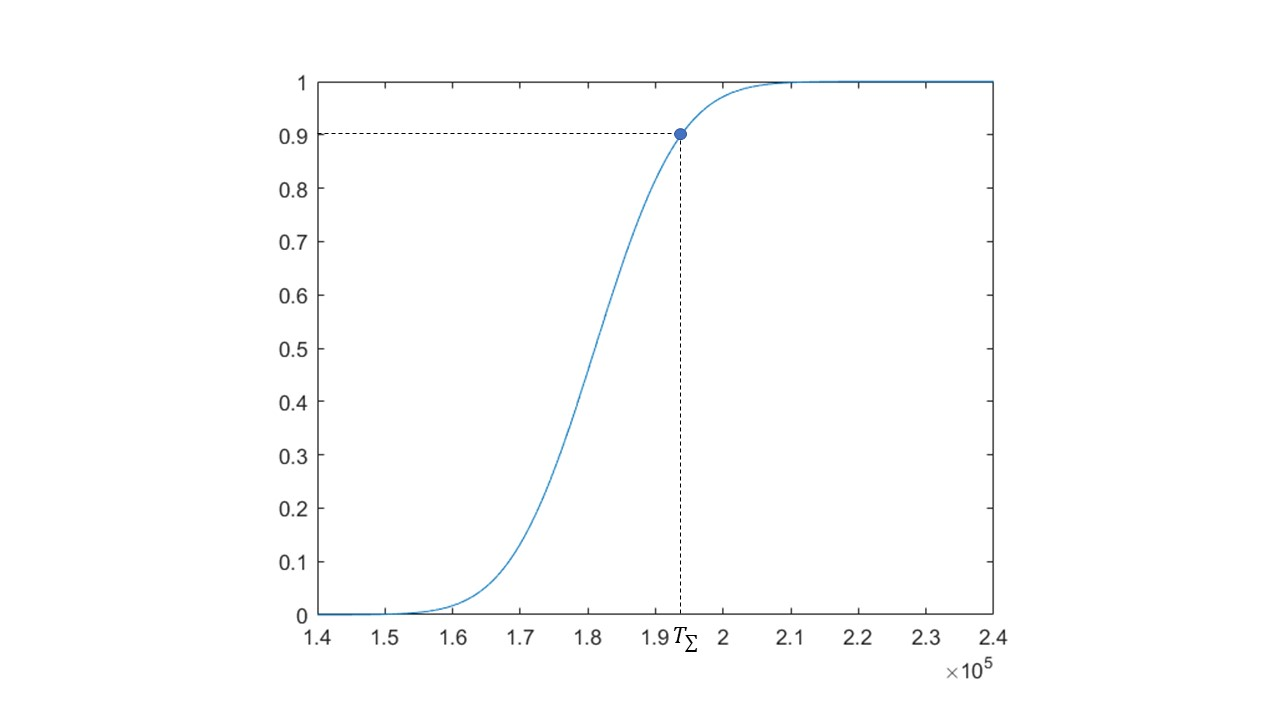
\includegraphics[scale=0.5]{正态2.jpg}
		\caption{总时间的概率分布函数}
	\end{figure}
	\qquad 用MATLAB有关正态函数对简化过后的积分方程进行求解,得到可靠性为90\%的前提下的最短时间,将最短时间变化为天数,即为最终答案。
	
	\qquad 最短天数为 $ T_{\Sigma}/16 = 134.5725 $,即需要至少135天。

	\subsection{问题五}
	\subsubsection{总体思路}
	由于每一种疫苗的生产用时不同、价格不同,因此其收益率各有差异。为达到最大销售额,各类型疫苗的产量应呈一定比例关系。比如:收益率高的疫苗比例大,可能全部生产;收益率低的比例小,可能不生产。因此我们需要确定能使得销售额最大的产量比例关系。
	\par 由之前的分析可知,以流水线方式生产疫苗,会产生等待时间。由于每种类型的生产任务可以拆分,因此可以通过合理安排疫苗的生产顺序来使得产量一定时的生产时间尽可能小。为了简化问题,我们分为两个步骤解决问题。假定疫苗生产用时没有随机性,其时间为均值。
	\par 首先,我们假定无等待时间,用线性规划求出在100天内达到最大销售额时各类型疫苗的总产量$N_{\Sigma 0}$。其总产量之比例可以看成是生产的比例。由于存在等待时间,因此实际的总产量必定小于线性规划求出的总产量。我们使用模拟退火算法求出最优的生产顺序,从而使得生产一批次的等待时间最少,进而其总产量最接近线性规划的总产量。
	\par 对于生产计划,我们以批为单位进行生产,一批中包含保持指定比例的各种疫苗。要在100天之内使生产批数最大。
	\subsubsection{用线性规划求解每种疫苗的产量比例}
	假定每个工位的生产无等待时间,则总时间为每种疫苗每箱用时的加权和。可以建立线性规划模型。
	\begin{itemize}
	\item 决策变量
	\par 决策变量为各类疫苗的产量
	\begin{equation}
		\boldsymbol{n}=\{n_{1},n_{2},\dots,n_{10}\}
	\end{equation}
	\item 目标函数
	\par 线性规划的优化目标是使得销售额最大。
	\begin{equation}
		M=\sum_{i}^{10}n_{i}m_{i}
	\end{equation}
	\item 约束条件
	\par 每种疫苗的产量应不大于任务数量。即
	\begin{equation}
		0\leqslant n_{i}\leqslant n_{i\max}(i\in\{1,2,\dots,10\})
	\end{equation}
	\par 在假定无等待时间的情况下,每个工位的生产时间应小于100天。即
	\begin{equation}
	\begin{split}
		&\sum_{i}^{10}n_{i}t(i,1)\leqslant T_{1\max}\\
		&\sum_{i}^{10}n_{i}t(i,2)\leqslant T_{2\max}\\
		&\sum_{i}^{10}n_{i}t(i,3)\leqslant T_{3\max}\\
		&\sum_{i}^{10}n_{i}t(i,4)\leqslant T_{4\max}\\
	\end{split}
	\end{equation}
	\item 优化模型
	\end{itemize}
	不考虑随机性,将均值即为每种疫苗的生产用时。总时间为
	\begin{equation}
	\begin{split}
		\max\quad &M=\sum_{i}^{10}n_{i}m_{i}\\
		s.t.\quad&0\leqslant n_{i}\leqslant n_{i\max}\quad i=1,2,\dots,10\\
		&\sum_{i}^{10}n_{i}t(i,j)\leqslant T_{j\max} \quad j=1,2,3,4\\
	\end{split}
	\end{equation}
	用matlab的线性规划函数求得产量结果如下表所示
	\begin{table}[H]
		\centering
		\caption{线性规划结果}\label{chanliang1}
		\begin{tabular}{ c| c| c |c|c|c|c|c|c|c|c}
			\hline
			疫苗 & YM1 & YM2 & YM3 & YM4 & YM5 & YM6 & YM7 & YM8 & YM9 & YM10 \\
			\hline
			 产量/剂 & 0 & 500 & 600 & 0 & 1200 & 1500 & 600 & 800 & 600 & 800 \\
			 \hline
		\end{tabular}
	\end{table}
	\par 由线性规划结果,我们得到每种类型的产量比例为
	\begin{equation}
	\begin{split}
	&n_1:n_2:n_3:n_4:n_5:n_6:n_7:n_8:n_9:n_{10}\\
	=&0:5:6:0:12:15:6:8:6:8
	\end{split}
	\end{equation}
	采用分批生产的方法,以一箱100剂为最小单位,一批中每种类型疫苗的生产箱数表示为$\boldsymbol{c}=(c_{1},c_{2},\dots,c_{10})$,其中$c_{i}$表示YM$i$在一批中的箱数。则可由产量比例得到每一批的产量分配:
	\begin{equation}
		\boldsymbol{c}=(0,5,6,0,12,15,6,8,6,8)
	\end{equation}
	考虑线性规划中忽略的等待时间后,其最终产量会有所减少,但疫苗如果按照这一比例生产,所得销售额仍应最大。我们运用模拟退火算法求解使产量最大的优化模型,得到最优的生产顺序。设定每一批的总疫苗箱数为66
	\par 以一个批次为单位进行生产
	优化目标为销售额
	线性规划
	模拟退火算法
	\subsubsection{确定生产顺序和总体产量}
	以一箱100个疫苗为基本单位
	\par 此问题的模拟退火算法与问题2类似,但是解空间不同。将每一箱作为排列中的每个元素,此时的解空间为66箱疫苗的排列$\boldsymbol{x}=(x_{1},x_{2},\dots,x_{66})$,排列中同一种疫苗根据产量比例可出现多次,即$\sum_{k}^{66}\boldsymbol{I}(x_{k}=$YM$i)=c_{i}$
	\par 求得生产顺序为()
	\par 每种疫苗的生产量如表\ref{chanliang2}所示,
	\begin{table}[H]	
		\centering
		\caption{每种疫苗的总产量}\label{chanliang2}
		\begin{tabular}{ c| c| c |c|c|c|c|c|c|c|c}
			\hline
			疫苗 & YM1 & YM2 & YM3 & YM4 & YM5 & YM6 & YM7 & YM8 & YM9 & YM10 \\
			\hline
			 产量/剂 & 0 & 490 & 588 & 0 & 1176 & 1470 & 588 & 784 & 588 & 784 \\
			 \hline
		\end{tabular}
	\end{table}
	对比表\ref{chanliang2}和表\ref{chanliang1}可知,最终优化了生产顺序的产量结果略小于忽略等待时间的结果。其最大销售额为$M_{max}=$
	
	\section{模型评价}
	\subsection{模型的优点}
	运用模拟退火算法,减小了搜索解的时间复杂度。
	\subsection{模型的不足}
	忽略的因素太多,不够精确
	\subsection{模型改进}
	
	\section{参考文献}
	%	\begin{thebibliography}{9}%宽度9
	%		\bibitem{bib:one} ....
	%	\end{thebibliography}
	
	\section{附录}
	\begin{appendices}
		
	\end{appendices}
	
\end{document}